\documentclass[10pt,twocolumn]{article}

\usepackage{amsthm}
\usepackage{comment}
\usepackage{amssymb}
\usepackage{amsmath}
\usepackage{fullpage}
\usepackage{graphicx}
\usepackage{multicol}
\usepackage{titlesec}
\usepackage{titling}
\usepackage[font={footnotesize,sf},labelfont={sf,bf},margin=1cm]{caption}
\usepackage[margin=0.55in]{geometry}
\footskip 20pt

\newtheoremstyle{ss}% hnamei
{3pt}% Space above
{3pt}% Space below
{\itshape}% Body font
{}% Indent amount
{\bfseries\sffamily}% Theorem head font
{:}% Punctuation after theorem head
{.5em}% Space after theorem head
{}% Theorem head spec (can be left empty, meaning `normal')
\theoremstyle{ss}
\newtheorem{rmk}{Remark}[section] 
\newtheorem{thm}{Theorem}[section] 

\pretitle{\begin{flushleft}\LARGE}
\posttitle{\par\end{flushleft}\vskip 0.5em}
\preauthor{\begin{flushleft}
\lineskip 0.5em%
\begin{tabular}{l}}
\postauthor{\end{tabular}\par\end{flushleft}}
\predate{\begin{flushleft}}
\postdate{\par\end{flushleft}}
\titleformat*{\section}{\large\bfseries\sffamily}
\titleformat*{\subsection}{\normalsize\bfseries\sffamily}

\usepackage{lmodern}
%\renewcommand*\familydefault{\sfdefault}
\newcommand{\lm}{\fontfamily{\sfdefault}\selectfont}
\newcommand{\mb}{\mathbf}

\usepackage{abstract}
\renewcommand{\abstractnamefont}{\bfseries\sffamily\normalsize}
%fg\renewcommand*{\abstractname}{\flushleft\textbf{}}

\title{\LARGE \bfseries \lm Control of Underactuated Vehicular Traffic}
\author{Stanislav Nikolov\\Massachusetts Institute of Technology\\July 12, 2012}
\date{}

\newenvironment{myindentpar}[1]%
 {\begin{list}{}%
         {\setlength{\leftmargin}{#1}}%
         \item[]%
 }
 {\end{list}}

\begin{document}

\twocolumn[
  \begin{@twocolumnfalse}
\maketitle
\vspace{-55pt}
\begin{myindentpar}{0.25cm}
\item 
\begin{paragraph}
\newline\noindent{\lm\bfseries Abstract:} We propose and study two control policies for the optimal velocity traffic model \cite{Bando} in which only an {\em active} subset of cars are actuated. We obtain sufficient conditions for the stability of the actuated dynamics and prove that in certain cases an unstable unactuated system can be stabilized. Through numerical experiments, we show that both controllers have a significant stabilizing effect. In particular, we study the number of active cars necessary to stabilize the dynamics, as well as the asymptotic convergence rate of each controller. We show that one controller is better when the unactuated dynamics are close to stable and the other is better when the unactuated dynamics are far from stable.
\end{paragraph}
\end{myindentpar}
\vspace{20pt}
\end{@twocolumnfalse}
]

% Misc stuff to talk about
% Traffic can actually smooth out by itself depending on the parameter governing the dynamics. Can show this analytically for linear dynamics, and demonstrate it for nonlinear dynamics.

% describe / motivate your system
\section{Introduction}
Traffic jams are a significant waste of gas and productivity and a source of great frustration. Traffic jams form for a variety of reasons. Disturbances, such as traffic accidents or road bottlenecks are a familiar and obvious cause. However, traffic jams are often observed to form spontaneously without any apparent disturbance. Even if all vehicles have the same velocity and headway (distance to the car in front), this configuration is often unstable. Drivers are not perfect, and under certain conditions, small disturbances in the headways and velocities are amplified, leading to a self-sustaining traffic jam. 

As robotic cars (such as Google's self-driving car \cite{Thrun}) being to join regular cars on the road in the near future, it is interesting to consider traffic as an underactuated dynamical system, and the problem of smoothing out traffic jams as an underactuated control problem. To investigate this, one must first study the dynamics of traffic without actuation, then design control policies to eliminate the traffic. %PLACEMENT!!!

theory of traffic jams has attracted a broad community of researchers and a diverse set of modeling approaches, including fluid models \cite{Kerner}, cellular automata models \cite{Benjaafar}, and car-following models \cite{Bando,Lenz,Liang00,Liang99,Yanakiev}. Here, we focus on car-following models and the vehicle dynamics that have been proposed to reproduce self-sustaining traffic jams. Bando et al. \cite{Bando} propose the optimal velocity model (OVM) and study the local linear stability about the uniform flow steady state. However, they consider only one type of car and do not consider control strategies. Lenz et al. \cite{Lenz} consider the stabilizing effect of an OV function that takes into account multiple headways.

In addition to models of the passive vehicle system, many have proposed control policies to smooth out traffic jams. Konishi et al. \cite{Konishi} studied the stability of an actuated OVM. Konishi's system is {\em fully-actuated} since one has control authority over each car. A more realistic scenario would be one in which the system is {\em underactuated}. In an underactuated vehicle system, one can only control a subset of {\em active} cars while the rest of the cars ({\em passive} cars) follow a given dynamics. Liang and Peng \cite{Liang00,Liang99} present a linear traffic model in which each vehicle regulates its headway using proportional-derivative control. They introduce a second type of car to model human drivers and characterize the stability of the mixed vehicle system. We propose an analogous system of mixed cars for the OVM model, as well as two control policies that stabilize an otherwise unstable system by controlling only the actuated subset of the cars.

\section{Car Following Model}
In order to talk about stabilizing vehicular traffic, we first present an idealized model of traffic flow. We model traffic as $N$ vehicles with positions $x_n$ and velocities $v_n$ driving counterclockwise on a single-lane circular road of circumference $L$.\footnote{A circular road may be thought of as an idealization of the circuit roads around many cities.} The cars are arranged such that car $i-1$ precedes car $i$. Each car has a headway (the free space in front) of $\Delta x_n$.

To model vehicle motion, we must model a driver's reaction to her vehicle's headway, and in particular, how the driver should accelerate or decelerate in response to the headway. Bando et al \cite{Bando} outline two popular reaction models --- the optimal distance model and the optimal velocity model. In the optimal distance model, the driver tries to regulate the headway to a desired value, accelerating if too far from the car in front and decelerating if too close. In the optimal velocity model, the driver tries to maintain an optimal velocity computed from the headway, accelerating when below the optimal velocity and decelerating when above it. We will consider the latter model, which has the following equations of motion:
\begin{align}
\label{ovm1} \dot{x}_n &= v_n,& &n=1,\dots,N\\
\label{ovm2} \dot{v}_n &= a\left(V(\Delta x_n) - v_n\right),& &n=1,\dots,N
\end{align}
where $a$ is the driver sensitivity and $V$ is the optimal velocity function. A common choice for $V$ \cite{Bando} is
\begin{gather*}
V(\Delta x)=\tanh(\Delta x - 2) + \tanh(2)
\end{gather*}

% SHOW GRAPH of V and V'
\begin{figure}[!h]
\lm
\begin{center}
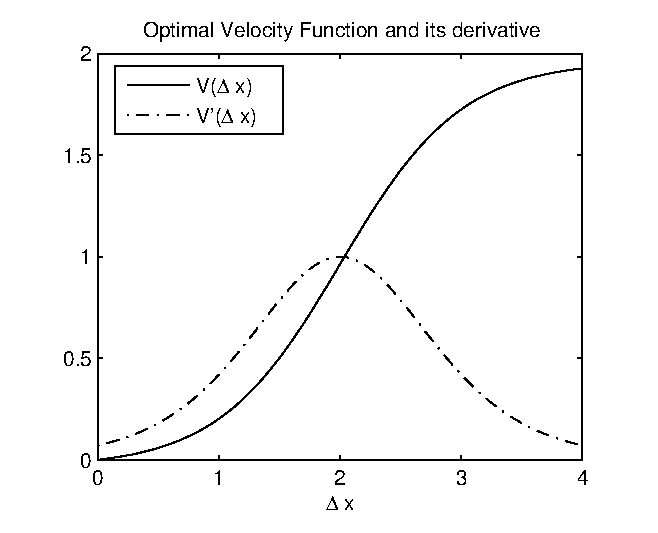
\includegraphics[width=3in]{vopt}
\end{center}
\caption{\label{fig:vopt} Optimal velocity function and its derivative.}
\end{figure}

Using this model, we can study the stability of uniform traffic flow.

\subsection{Linear Stability Analysis}
It is clear that the OVM equations of motion are satisfied when there is uniform traffic flow, i.e. when all cars have headway $L/N$ and velocity $V(L/N)$. In terms of car positions, this can be expressed as
\begin{gather}
x_n^*=bn + V(b)t
\intertext{where}
b=\frac{L}{N}
\end{gather}
This represents a fixed point in headway-velocity space. To study the stability of this fixed point, we express $x_n$ as the uniform flow steady state $x_n^*$ plus some perturbation $y_n$
\begin{gather}
x_n=x_n^*+y_n.
\end{gather}
Linearizing (\ref{ovm1}) and (\ref{ovm2}) and observing that $\dot{y}_n=\dot{x}_n$ and $\ddot{y}_n=\ddot{x}_n$ gives us the linearized equation for $y_n$
\begin{gather}
\label{ovml} \ddot{y}_n = a\left(f\Delta y_n - \dot{y}_n \right)
\intertext{where $f$ is the derivative of $V$ at the uniform flow headway $b$}
f=V'(b).
\end{gather}
We solve (\ref{ovml}) by considering as solutions the time-evolving discrete Fourier modes
\begin{gather}
y_k(n,t)=\exp\left(i\alpha_k n + zt\right)\\
\alpha_k = \frac{2\pi}{N}k (k=0,1,\dots,N-1)
\intertext{where}
z=u+iv
\intertext{and $u$ and $v$ are real.}
\end{gather}
Plugging $y_k(n,t)$ into (\ref{ovml}), we get a condition on $a,z,f$ and $\alpha_k$:
\begin{gather}
\label{zcond} z^2 + az - af\left(e^{-i\alpha_k} - 1\right) = 0
\end{gather}
Each mode $e^{i\alpha_kn}$ represents a spatial wave of car positions (relative to uniform flow) and evolves in time according to $z$. The uniform flow fixed point is stable whenever each of the $N$ spatial modes decays, i.e. whenever the real part of $z$ is negative for all $k$. Let us characterize the values of $a$ and $f$ for which this is the case. 
\begin{thm}
The unactuated system is stable if and only if $f < a/2$.
\end{thm}
\begin{proof}
Expanding (\ref{zcond}) and treating the real and imaginary parts separately, we get
\begin{gather}
\label{stbl1} u^2 + au + af(1 - \cos(\alpha_k) ) - v^2\\
\label{stbl2} 2uv + av + af\sin(\alpha_k) = 0. 
\end{gather}
Solving (\ref{stbl1}) for $u$ and requiring $u<0$ gives
\begin{gather}
u = \frac{-a \pm \sqrt{a^2 - 4(af(1-\cos(\alpha_k))-v^2)}}{2} < 0
\end{gather}
\begin{align}
 a^2 - 4(af(1-\cos(\alpha_k))-v^2) &< a^2\\
 - 4(af(1-\cos(\alpha_k))-v^2) &< 0\\
\label{stbl3}  af(1-\cos(\alpha_k)) &> v^2
\end{align}
In (\ref{stbl3}), $v$ is unknown, but solving (\ref{stbl2}) for $u$ and requiring $u<0$ will give us a bound on $v$. From (\ref{stbl2}), we get
\begin{gather}
u = \frac{-af\sin(\alpha_k)-av}{2v} < 0.
\end{gather}
Rearranging, we arrive at
\begin{gather}
-\frac{f\sin(\alpha_k)}{v} < 1.
\end{gather}
Replacing $v$ with its absolute value yields
\begin{align}
|v|&>-f\sin(\alpha_k),& &v \geq 0\\
|v|&>f\sin(\alpha_k),& &v<0
\end{align}
and finally, gives a bound on $v^2$
\begin{gather}
\label{stbl4} v^2 > f^2\sin^2(\alpha_k).
\end{gather}

Combining (\ref{stbl3}) and (\ref{stbl4}) results in
\begin{align}
af(1-\cos(\alpha_k)) &> f^2\sin^2(\alpha_k)\\
 f &< \frac{a(1-\cos(\alpha_k))}{\sin^2(\alpha_k)}\\
 f &< \frac{a(1-\cos(\alpha_k))}{1-\cos^2(\alpha_k)}\\
 f &< \frac{a(1-\cos(\alpha_k))}{(1+\cos(\alpha_k))(1-\cos(\alpha_k))}\\
\label{stbl5}  f &< \frac{a}{2\cos^2(\frac{\alpha_k}{2})}.
\end{align}
Recalling that the uniform flow is not stable unless (\ref{stbl5}) is true for all $k$, we get a simple necessary and sufficient stability condition on $a$ and $f$:
\begin{gather}
f < \frac{a}{2}
\end{gather}
\end{proof}

This result is summarized visually in Figure \ref{fig:stblregion}.

\begin{figure}[!h]
\lm
\begin{center}
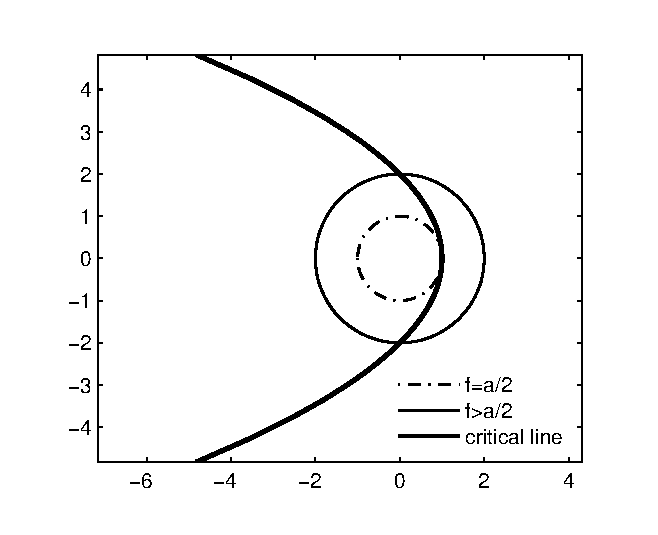
\includegraphics[width=3in]{stblregion}
\end{center}
\caption{ \label{fig:stblregion} The stability of the uniform flow fixed point is characterized by a critical line in the $(f,\alpha)$ plane in polar coordinates. Here, $\alpha$ is taken to be a continuous parameter for simplicity.}
\end{figure}

\section{Analysis of Control Policies}
Suppose that we can control a subset of the cars. In this section, we propose two control policies --- {\em caution function control} and {\em velocity matching control} --- and study their stability.

\subsection{Control Using Caution Functions}
Let us call the cars we can control {\em active} and the rest of the cars {\em passive}. Let $\mathcal{A}$ be the set of active car indices and $\mathcal{P}$ be the set of passive car indices. 

Consider the following control policy for active cars. Whenever an active car has headway $\Delta x$, its driver pretends that the headway is actually $c(\Delta x)$, where $c$ is a {\em caution function} that is nonnegative, sublinear, monotonically increasing, and differentiable on $(0,\infty)$. The car then follows the optimal velocity dynamics as usual. The modified dynamics are
\begin{align}
\dot{x}_n &= v_n,& &n=1, \dots, N\\
\dot{v}_n &= a\left(V(\Delta x_n) - v_n \right),& &n \in \mathcal{P}\\
\dot{v}_n &= a\left(V(c(\Delta x_n)) - v_n \right),& &n \in \mathcal{A}.
\end{align}
or in headway-velocity space,
\begin{align}
&\dot{\Delta x}_n = v_{n-1}-v_n,& &n=1,\dots, N\\
&\dot{v}_n = a\left(V(\Delta x_n) - v_n \right),& &n \in \mathcal{P}\\
&\dot{v}_n = a\left(V(c(\Delta x_n)) - v_n \right),& &n \in \mathcal{A}
\end{align}
Now let us find the fixed point of these dynamics in headway-velocity space and analyze its stability. Setting $\dot{\Delta x}_n$ and $\dot{v}_n$ to 0, we get
\begin{align}
&\label{cfp1} v_{n-1}^* = v_n^*,& &n=1, \dots, N\\
&v_n^* = V(\Delta x_n^*),& &n \in \mathcal{P}\\
&v_n^* = V(c(\Delta x_n^*)),& &n \in \mathcal{A}
\end{align}
Let us now consider two adjacent cars $p$ and $a$, with the $p$th passive and the $a$th active. Because their velocities must be equal we have 
\begin{gather}
V(\Delta x_p^*)=V(c(\Delta x_a^*)).
\intertext{For monotonic $V$, this implies}
\label{cfp2} \Delta x_p^*=c(\Delta x_a^*).
\end{gather}
Because adjacent cars of the same type have the same velocity, and hence headway, all the passive cars have headway $\Delta x_p^*$ and all the active cars have headway $\Delta x_a^* = c(\Delta x_p^*)$. Equations (\ref{cfp1}) and (\ref{cfp2}), together with the constraint $\sum_{n=1}^N \Delta x_n = L$ then determine the fixed point.

To linearize around the fixed point, it will prove useful to represent the state as the deviation of each headway from the desired headway, and the difference in velocities of adjacent cars
\begin{gather}
y_n = x_{n-1} - x_n - \Delta x_n^*\\
w_n = v_{n-1} - v{n}
\end{gather}
giving dynamics
\begin{gather}
\dot{y}_n = w_n, \; n=1,\dots, N\\
\dot{w}_n = a\left(V_{n-1}(y_{n-1} + \Delta x_{n-1}^*) - V_n(y_n + \Delta x_n^*) - w_n \right)
\end{gather}
where $V_n = V$ for $n \in \mathcal{P}$ and $V_n = V \circ c$ for $n \in \mathcal{A}$. Note that the $y$ here is different from the $y$ used in the unactuated case. The linearized dynamics are
\begin{align}
\label{cfdyn} \ddot{y}_n &= a(f_{n-1}y_{n-1} - f_n y_n - \dot{y}_n)
\end{align}
where
\begin{align}
f_n &= f_p = V'(\Delta x_p^*), \; n \in \mathcal{P}
\intertext{and}
f_n = f_a &= V'(c(\Delta x_a^*))c'(\Delta x_a^*), \; n \in \mathcal{A}\\
&= V'(\Delta x_p^*) c'(\Delta x_a^*)\\
&= f_p \sigma.
\end{align}
Note that we cannot assume solutions of the form $y_k(n,t)=\exp\left(i\alpha_kn + zt\right)$ like we could in the unactuated case. To see this, observe that plugging $y_k(n,t)$ into the four cases of the dynamics in Equation (\ref{cfdyn}) yields unsatisfiable conditions on $z$. Indeed, this is because $y_k(n,t)$ are eigenvectors of the linearized unactuated dynamics but not of the linearized actuated dynamics. \footnote{The issue here is that the unactuated dynamics have only one type of car, and this makes the linearized system simple enough to allow one to guess that its eigenvectors are $y_k(n,t)$. The nonuniformity introduced by active cars makes it far more difficult to determine the eigenvectors of the linearized actuated system.}

Hence, we study stability using the {\em string stability} framework of \cite{Liang00,Liang99}, \cite{Konishi} and \cite{Yanakiev}. In this framework, we look at how disturbances in headway (relative to the steady-state headway) propagate between consecutive cars by investigating the transfer function of the dynamics in Equation (\ref{cfdyn})
\begin{gather}
s^2 Y_n(s) = a(f_{n_1}Y_{n-1}(s) - f_nY_n(s) - sY_n(s))\\
Y_n(s) = \frac{af_{n-1}}{s^2 + as + af_n}Y_{n-1}(s)\\
Y_n(s) = G_{n-1,n}(s)Y_{n-1}(s).
\end{gather}
To see what happens for a full cycle of propagation, we can relate $Y_N(s)$ to $Y_1(s)$ by writing
\begin{align}
Y_N(s) &= G_{1,N}(s) Y_1(s)\\
&= G_{1,2}(s) \dots G_{N-1,N}(s) Y_1(s).
\end{align}
The system is stable if and only if
\begin{enumerate}
\item for all $n$, $G_{n-1,n}(s)$ has no poles
\item $\|G_{1,N}(j\omega)\|_{\infty} := \displaystyle \sup_{\omega \in [0,\infty)} |G_{1,N}(j\omega)| \leq 1$.
\end{enumerate}
The first condition ensures that the system doesn't blow up due to a pole. The second condition ensures that disturbances in headway are not amplified indefinitely as cars go around the circular road.
Let us compute the magnitude and sup-norm of $G_{n-1,n}(j\omega)$.
\begin{align}
|G_{n-1,n}(j\omega)| &= \sqrt{G_{n-1,n}(j\omega)G_{n-1,n}(-j\omega)}\\
&= \sqrt{\frac{a^2f_{n-1}^2}{(af_n - \omega^2)^2 + a^2\omega^2}}
\end{align}

There are four cases of $|G_{n-1,n}(j\omega)|$ depending on $f_n$ and $f_{n-1}$:
\begin{align}
|G_{a,a}(j\omega)| &= \sqrt{\frac{a^2f_p^2\sigma^2}{(af_p\sigma - \omega^2)^2 + a^2\omega^2}}\\
|G_{p,a}(j\omega)| &= \sqrt{\frac{a^2f_p^2}{(af_p\sigma - \omega^2)^2 + a^2\omega^2}}\\
|G_{a,p}(j\omega)| &= \sqrt{\frac{a^2f_p^2\sigma^2}{(af_p - \omega^2)^2 + a^2\omega^2}}\\
|G_{p,p}(j\omega)| &= \sqrt{\frac{a^2f_p^2}{(af_p - \omega^2)^2 + a^2\omega^2}}.
\end{align}
Here, we have abused notation to indicate the transfer functions between adjacent passive or active cars.
The amplitude of the full-cycle transfer function $G_{1,N}$ can then be written as
\begin{align*}
|G_{1,N}(j\omega)| = |G_{a,a}(j\omega)|^{N_{a,a}} &\cdot |G_{p,a}(j\omega)|^{N_{p,a}} \cdot \\ |G_{a,p}(j\omega)|^{N_{a,p}} &\cdot |G_{p,p}(j\omega)|^{N_{p,p}}
\end{align*}
where $N_{*,*}$ indicates the number of instances of each type of pair of adjacent cars.
\begin{thm}
If $f_p < a/2$, the actuated system is stable.
\end{thm}
\begin{proof}
Assuming no poles, a sufficient condition for stability is
\begin{align*}
\|G_{a,a}\|_{\infty}^{N_{a,a}} \cdot \|G_{p,a}\|_{\infty}^{N_{p,a}} \cdot \|G_{a,p}\|_{\infty}^{N_{a,p}} \cdot \|G_{p,p}\|_{\infty}^{N_{p,p}} \leq 1.
\end{align*}
Konishi \cite{Konishi} showed that for a system of passive cars, $|G_{n-1,n}(j\omega)|$ achieves only a single maximum at $\omega=0$ if $f < a/2$. This corresponds to $\partial |G_{n-1,n}(j\omega)|/\partial \omega$ having only one real root. Adapting this result to the mixed-car case gives $f_p < a/2$ and $f_p\sigma < a/2$, the latter of which is implied by the former due to the definition of the caution function. This allows us to compute the sup-norms simply by evaluating the amplitudes at $\omega=0$:
\begin{align*}
\|G_{a,a}\|_{\infty} &= 1\\
\|G_{p,a}\|_{\infty} &= 1/\sigma\\
\|G_{a,p}\|_{\infty} &= \sigma\\
\|G_{p,p}\|_{\infty} &= 1.
\end{align*}
It is clear then that for $f_p < a/2$, disturbances are not amplified:
\begin{gather}
\|G_{1,N}\|_{\infty} \leq\\
\|G_{a,a}\|_{\infty}^{N_{a,a}} \cdot \|G_{p,a}\|_{\infty}^{N_{p,a}} \cdot \|G_{a,p}\|_{\infty}^{N_{a,p}} \cdot \|G_{p,p}\|_{\infty}^{N_{p,p}} \\
= 1^{N_{a,a}} \cdot \left(\frac{1}{\sigma}\right)^{N_{p,a}} \cdot \sigma^{N_{a,p}} \cdot 1^{N_{p,p}} \\
\leq 1.
\end{gather}
The condition $f_p < a/2$ also implies that there are no poles (see Konishi \cite{Konishi} for details). Hence, we conclude that $f_p < a/2$ is a sufficient condition for stability.
\end{proof}
This leads us to a key result.
\begin{rmk}
Caution function control can increase the region of stability.\footnote{Note that the region of stability --- the region in paramter space for which the system is stable, is different from the region of {\em attraction} --- the region in state space of all initial conditions that convergence to the fixed point.}
\end{rmk}
Observe that for a given car density $b$, caution function control results in the optimal headways 
\begin{gather}
\Delta x_p^* < b < \Delta x_a^*.
\end{gather}
For $b \leq 2$ (the inflection point of $V$), this implies
\begin{gather}
f_p = V'(\Delta x_p^*) < V'(b) = f
\end{gather}
This results in cases in which the unactuated system is unstable ($f > a/2$), but the caution-function-actuated system is stable ($f_p < a/2$). This phenomenon is illustrated in Figure \ref{fig:ctrstbl}. Because we only showed $f_p < a/2$ to be a sufficient condition, we cannot conclude anything about the relative stability of the actuated and unactuated systems if $b>2$. However, we show numerically in Section \ref{sec:numer} that caution function control has a stabilizing effect even when $b>2$. 

\begin{figure}[!h]
\begin{center}
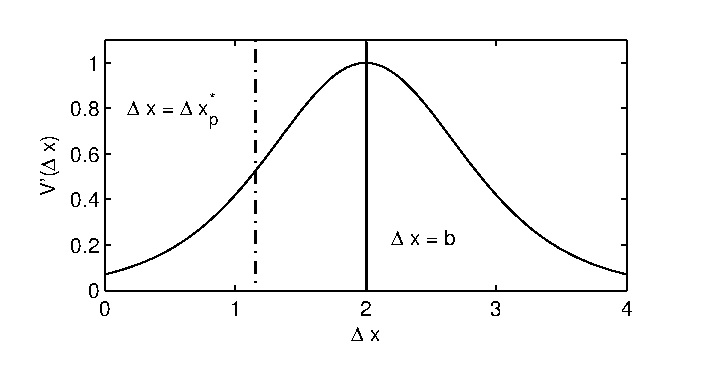
\includegraphics[width=3in]{vopt_caution}
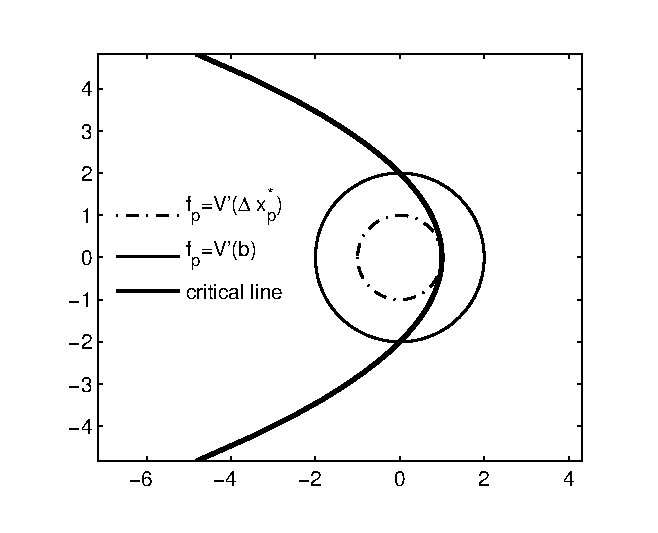
\includegraphics[width=3in]{ctrstbl}
\end{center}
\caption{ \label{fig:ctrstbl} The caution function pushes $V'$ down so that $f_p$ moves from the unstable region to the stable region.}
\end{figure}

\subsection{Control Using Velocity Matching}
Another control strategy is for the active cars to try to match the velocity of the preceding vehicle in addition to the optimal velocity prescribed by the headway. We proceed in a manner similar to that of the previous section to obtain a sufficient condition for stability. Unfortunately, this results in conditions that are at least as restrictive as those in the unactuated case. That is, we cannot conclude that the region of stability for the actuated system is any larger than that of the unactuated system. 

The equations of motion for velocity-matching control in headway-velocity space are
\begin{align}
&\dot{\Delta x}_n = v_{n-1} - v_n,& &n=1, \dots, N\\
&\dot{v}_n = a\left(V(\Delta x_n) - v_n \right),& &n \in \mathcal{P}\\
&\dot{v}_n = a\left(V(\Delta x_n) - v_n \right) + k(v_{n-1}-v_n),& &n \in \mathcal{A}
\end{align}
Observe that the fixed point is $\Delta x_n^* = b, v_n = V(b)$ for $n=1,\dots,N$, the same as that of the unactuated system. Let us investigate its region of stability and how it compares to that of the unactuated system. As with caution function control, we use the state space representation $y_n = x_{n-1} - x_n - \Delta x_n^*, w_n = v_{n-1} - v_n$. This gives the following dynamics, which depends on the type of cars at the $n$th and $n-1$th positions:
\begin{gather*}
\ddot{y}_n = a(V(y_{n-1} + \Delta x_{n-1}^*)y_{n-1} - V(y_n + \Delta x_{n}^*)y_n - \dot{y}_n) \\ + k\dot{y}_{n-1} - k\dot{y}_n
\end{gather*}
for $n-1 \in \mathcal{A}, n \in \mathcal{A}$,
\begin{gather*}
\ddot{y}_n = a(V(y_{n-1} + \Delta x_{n-1}^*)y_{n-1} - V(y_n + \Delta x_{n}^*)y_n - \dot{y}_n) \\ - k\dot{y}_n
\end{gather*}
for $n-1 \in \mathcal{P}, n \in \mathcal{A}$,
\begin{gather*}
\ddot{y}_n = a(V(y_{n-1} + \Delta x_{n-1}^*)y_{n-1} - V(y_n + \Delta x_{n}^*)y_n - \dot{y}_n) \\ + k\dot{y}_{n-1}
\end{gather*}
for $n-1 \in \mathcal{A}, n \in \mathcal{P}$, and
\begin{gather*}
\ddot{y}_n = a(V(y_{n-1} + \Delta x_{n-1}^*)y_{n-1} - V(y_n + \Delta x_{n}^*)y_n - \dot{y}_n)
\end{gather*}
for $n-1 \in \mathcal{P}, n \in \mathcal{P}$.


Linearizing about $y_n=0$ gives
\begin{gather*}
\ddot{y}_n = a(f(y_{n-1} - y_n) - \dot{y}_n) + k\dot{y}_{n-1} - k\dot{y}_n
\end{gather*}
for $n-1 \in \mathcal{A}, n \in \mathcal{A}$,
\begin{gather*}
\ddot{y}_n = a(f(y_{n-1} - y_n) - \dot{y}_n) - k\dot{y}_n
\end{gather*}
for $n-1 \in \mathcal{P}, n \in \mathcal{A}$,
\begin{gather*}
\ddot{y}_n = a(f(y_{n-1} - y_n) - \dot{y}_n) + k\dot{y}_{n-1}
\end{gather*}
for $n-1 \in \mathcal{A}, n \in \mathcal{P}$, and
\begin{gather*}
\ddot{y}_n = a(f(y_{n-1} - y_n) - \dot{y}_n)
\end{gather*}
for $n-1 \in \mathcal{P}, n \in \mathcal{P}$.

Proceeding like we did for caution function control in the previous section, we find the transfer functions $G_{a,a}(s)$, $G_{a,p}(s)$, $G_{p,a}(s)$, $G_{p,a}(s)$ that describe how disturbances propagate across each type of adjacent car pair. They are
\begin{align}
G_{a,a}(s) &= \frac{af + ks}{s^2 + (a+k)s + af}\\
G_{p,a}(s) &= \frac{af}{s^2 + (a+k)s + af}\\
G_{a,p}(s) &= \frac{af + ks}{s^2 + (a)s + af}\\
G_{p,p}(s) &= \frac{af}{s^2 + as + af}
\end{align}
and they have magnitudes
\begin{align}
|G_{a,a}(j\omega)| &= \frac{a^2f^2 + k^2\omega^2}{(af - \omega^2)^2 + (a+k)^2\omega^2}\\
|G_{p,a}(j\omega)| &= \frac{a^2f^2}{(af - \omega^2)^2 + (a+k)^2\omega^2}\\
|G_{a,p}(j\omega)| &= \frac{a^2f^2 + k^2\omega^2}{(af - \omega^2)^2 + a^2\omega^2}\\
|G_{p,p}(j\omega)| &= \frac{a^2f^2}{(af - \omega^2)^2 + a^2\omega^2}
\end{align}

To obtain a sufficient condition for stability, we can again require that there are no poles, and that the $|G_{*,*}(j\omega)|$ all attain their maximum value at $\omega=0$. However, as far as proving that a system actuated by velocity matching has a larger region of stability than an unactuated system, this approach would prove futile. An examination of $|G_{p,p}(j\omega)|$ reveals that there are no poles if only if $f < a/2$, just like in the case of caution function control, whose corresponding $G_{p,p}(j\omega)$ transfer function has the same denominator. This is already the stability condition for the unactuated system, and any further conditions we derive with this approach can only cause more restrictions. 

Although we cannot conclude that velocity matching control enlarges the region of stability, the velocity matching policy is still useful. In section \ref{sec:numer}, we show numerically that velocity matching control results in dynamics with faster convergence and in fact, has a larger region of stability than the unactuated system.

\section{Numerical Simulations}
\label{sec:numer}

We investigate numerically the stability of the unactuated system and the stabilizing effect of velocity matching control and caution function control. For all simulations, unless stated otherwise, the road is of length $L=200$ and there are $N=100$ cars.

\subsection{Stability Threshold of Unactuated System}
We demonstrate the behavior of the unactuated system around the threshold for stability. Figure \ref{fig:instability2} shows a typical unstable system using a spatiotemporal diagram.

\begin{figure}[!h]
\begin{center}
\includegraphics[width=3in]{traffic4}
\end{center}
\caption{ \label{fig:instability2} A spatiotemporal diagram of an unstable traffic system initialized at the steady state except for a single car moving with positive velocity. The y-axis is time and the x-axis is position. Notice the merging of small traffic jams into bigger ones as time goes by.}
\end{figure}

The condition for stability for $L/N=2$ is $a > 2f = 2$. Figure \ref{fig:instability} shows the time evolution of an unstable system with $a<2$ and Figure \ref{fig:smoothed} shows the time evolution of a stable system for $a>2$.

\begin{figure}[!h]
\begin{center}
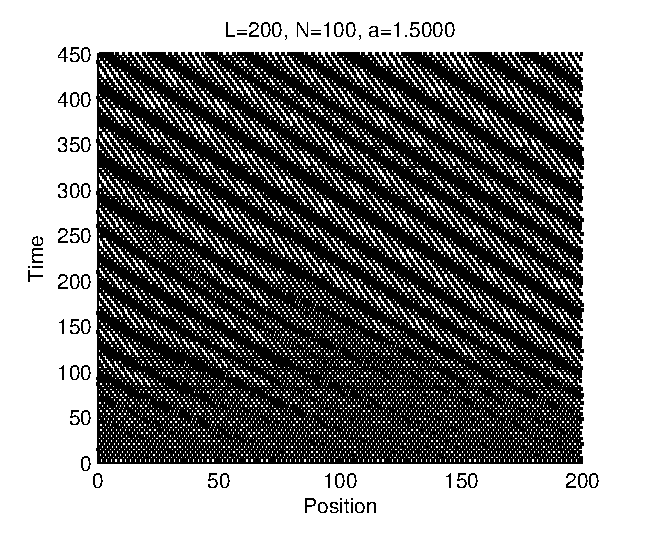
\includegraphics[width=3in]{instability}
\end{center}
\caption{ \label{fig:instability} For sensitivity $a<2f$, the uniform traffic flow configuration is unstable. Starting a small perturbation from uniform flow, the system is pushed away toward a self sustaining traffic jam.}
\end{figure}

\begin{figure}[!h]
\begin{center}
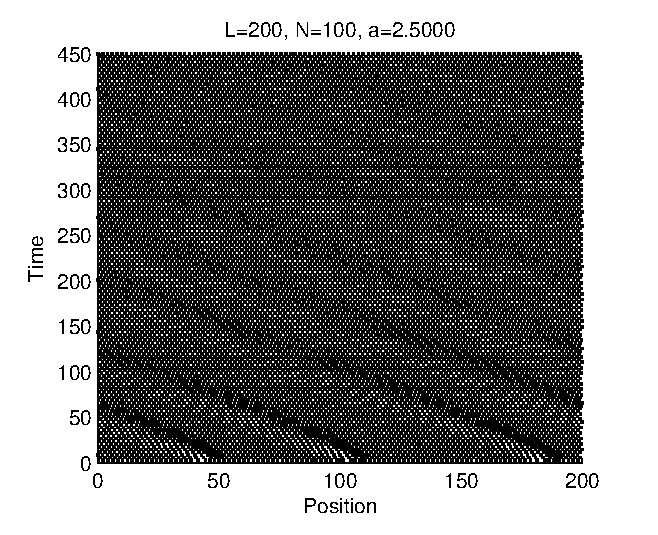
\includegraphics[width=3in]{smoothed}
\end{center}
\caption{ \label{fig:smoothed} For sensitivity $a>2f$, the uniform traffic flow configuration is stable. Starting a small perturbation from uniform flow, the disturbances in the vehicle velocities and headways are smoothed out.}
\end{figure}

Figure \ref{fig:typinst} shows a plot of headways for a typical unstable system.

\begin{figure}[!h]
\begin{center}
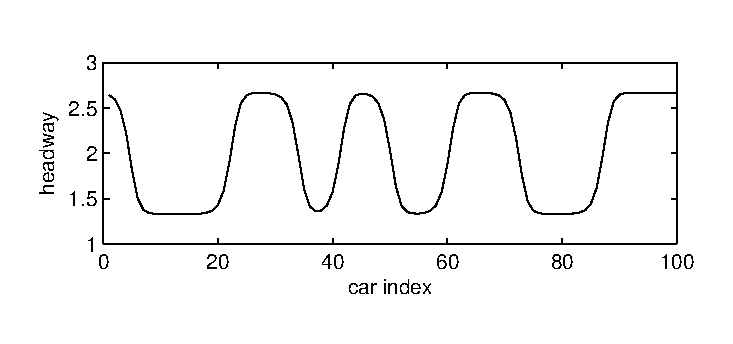
\includegraphics[width=3in]{typinst}
\end{center}
\caption{ \label{fig:typinst} Headways in a typical unstable system.}
\end{figure}

\subsection{Stabilizing Effect of Control Policies}
We investigate and compare the stabilizing effect of velocity matching control and caution function control. In each experiment, the system is initialized so that each headway and velocity is perturbed from the steady-state velocity and headway with uniform noise between $-0.025$ and $0.025$. For velocity matching control, we use gains $k=1$ and $k=10$. For caution function control, we use caution functions $c(\Delta x) = \Delta x^{0.5}$ and $c(\Delta x) = \Delta x^{0.25}$. Note that although these choices of $c$ only sublinear for $\Delta x > 1$, this is always the case for the parameters chosen.

We first study how many active cars are needed to stabilize the system for each type of control. We consider two types of active car configurations --- equidistant and block. In the equidistant configuration, we pick a number $\ell$ and make every $\ell$th car active, which gives $\lceil \frac{N}{\ell} \rceil$ cars. Hence, the possible number of active cars is $N, \lceil \frac{N}{2} \rceil, \lceil \frac{N}{3} \rceil, \dots$. In the block configuration, we simply put all the active cars in a contiguous block. Table \ref{tbl:stbl} shows the number of cars necessary to stabilize a system with $a=1.5$ and a system with $a=1$ in both block and equidistant configurations.

\begin{table}[h!]
\footnotesize
\begin{center}
\begin{tabular}{|l|cc|cc|}
\multicolumn{5}{c}{$b=2$ (unactuated system is stable for $a > 2$)}\\\hline
& \multicolumn{2}{c}{$a=1.5$} & \multicolumn{2}{c}{$a=1.0$}\\\hline
& Equidist. & Block & Equidist. & Block\\\hline
vel. match. ($k=1$) & 25 & 24 & 50 & 50\\
vel. match. ($k=10$) & 25 & 22 & 100 & 69\\
caution func. ($\Delta x^{0.5}$) & 5 & 4 & 15 & 22\\
caution func. ($\Delta x^{0.25}$) & 2 & 2 & 5 & 5\\
\hline
\multicolumn{5}{c}{$b=2.5$ (unactuated system is stable for $a > 1.57$)}\\\hline
& \multicolumn{2}{c}{$a=1.5$} & \multicolumn{2}{c}{$a=1.0$}\\\hline
& Equidist. & Block & Equidist. & Block\\\hline
vel. match. ($k=1$) & 2 & 2 & 34 & 43\\
vel. match. ($k=10$) & 1 & 1 & 50 & 45\\
caution func. ($\Delta x^{0.5}$) & 3 & 4 & 14 & 12\\
caution func. ($\Delta x^{0.25}$) & 1 & 1 & 5 & 5\\
\hline
\end{tabular}
\end{center}
\caption{\label{tbl:stbl} The minimum number of cars necessary to stabilize a system with $a=1.5$ and $a=1.0$. Above: $b=2$. Both values of $a$ are far from the threshold. Below: $b=2.5$. One value of $a$ is close to the threshold while the other is far from it. Note that the number of cars in an equidistant configuration can only be $N, \lceil \frac{N}{2} \rceil, \lceil \frac{N}{3} \rceil, \dots$. Hence, a minimum of 100 cars reflects that the next possibility of 50 cars is insufficient for stability.}
\end{table}

We also investigated the asymptotic rates of convergence for the actuated and unactuated systems. Figure \ref{fig:convscl5} compares the convergence rates for 20 active cars out of 100. Figure \ref{fig:convscl25} does the same for 4 active cars out of 100. To ensure stability for all systems, actuated or not, the value of $a$ is set to 2.1.
\begin{figure}[!h]
\lm
\begin{center}
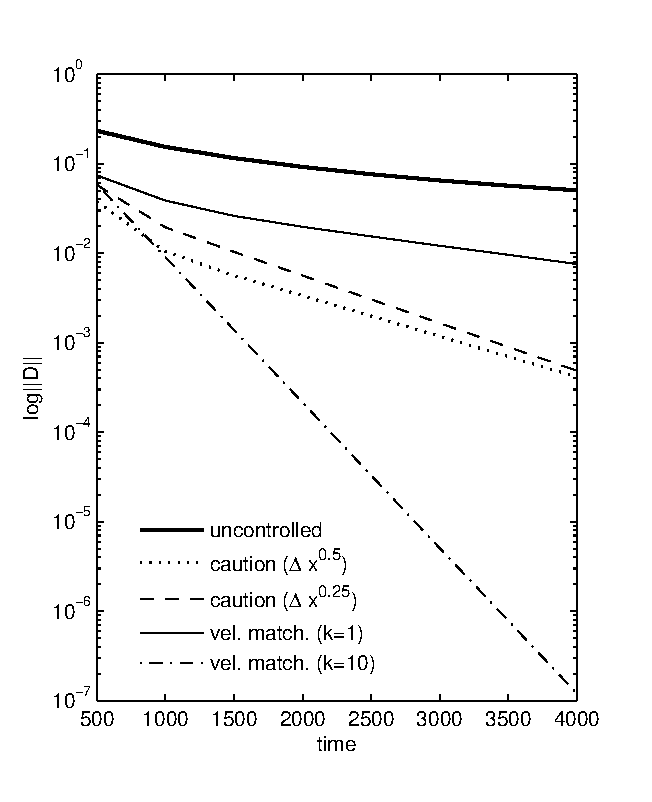
\includegraphics[width=3in]{convscl5}
\end{center}
\caption{ \label{fig:convscl5} Convergence rates for different control policies represented by the time evolution of the $\ell^2$ norm of the discrete Fourier transform of headways relative to the fixed point headways. There are 100 cars on a road of circumference 200, and the car sensitivities are $a=2.1$ (just above the stability threshold for the unactuated system). All the systems are stable but the actuated systems converge much faster. There are 20 active cars in an equidistant configuration. A high-gain velocity matching controllers vastly outperforms the caution function controllers.}
\end{figure}
\begin{figure}[!h]
\lm
\begin{center}
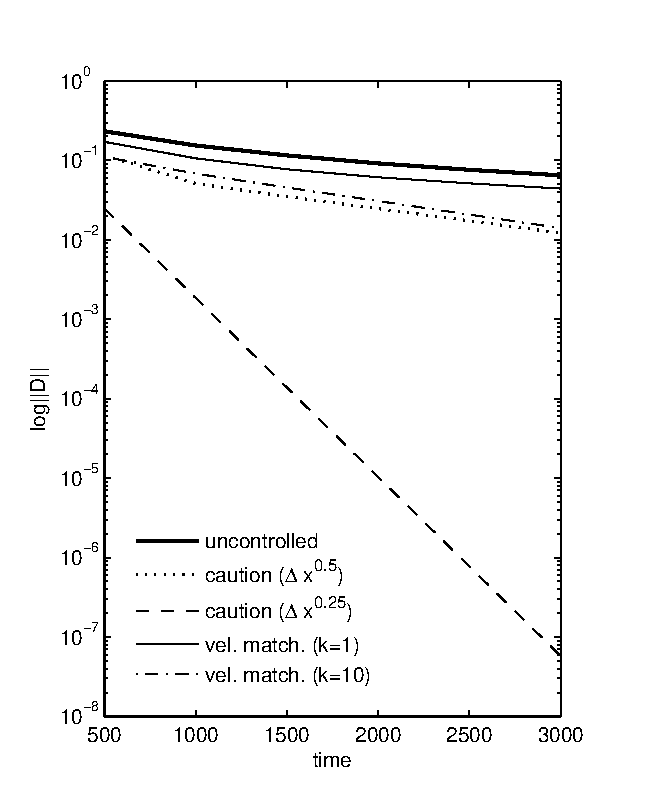
\includegraphics[width=3in]{convscl25}
\end{center}
\caption{ \label{fig:convscl25} Convergence rates for different control policies (see Figure \ref{fig:convscl5}) There are 4 active cars in an equidistant configuration. The smaller number of active cars allows for higher steady-state headways for the active cars and lower steady-state headways for the passive cars, enlarging the region of stability (c.f. Figure \ref{fig:ctrstbl}).}
\end{figure}

Figure \ref{fig:absfft} shows another view of convergence rates. Depicted are the amplitudes of the Fourier transform of the headways over time. We see that both increasing the gain $k$ and the number of cars increases stability for velocity matching control (although we observed instability for high enough gain).
\begin{figure}[!h]
\lm
\begin{center}
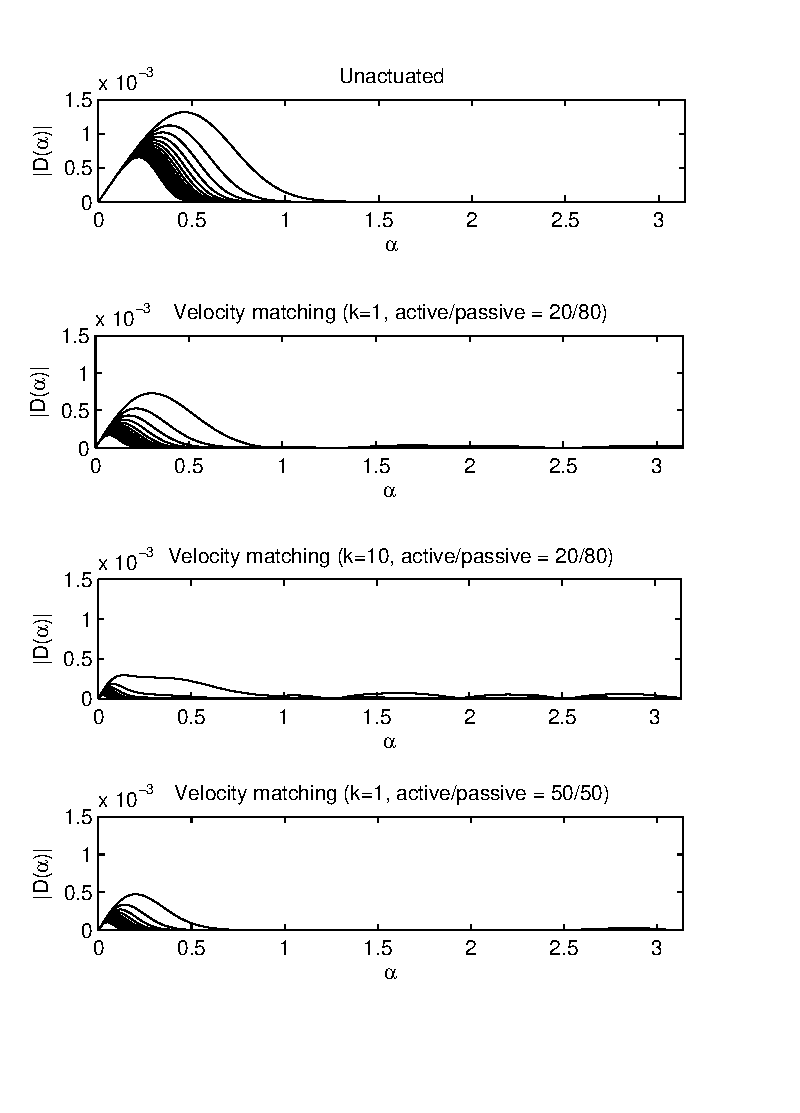
\includegraphics[width=3in]{absfft}
\end{center}
\caption{ \label{fig:absfft} The amplitude of the Fourier transform of the headways decays over time for a stable system. For velocity matching control, a higher gain $k$ and a higher number of active cars (in equidistant configurations) speed up this decay.}
\end{figure}

\section{Discussion and Future Work}

\subsection{Main Results}
For velocity matching control, higher gain appears to reduce the stabilizing effect when the unactuated system is far from stable. Table \ref{tbl:stbl} shows that for $a=1$, a gain of $k=1$ requires fewer cars to stabilize the system than a gain of $k=10$ in all cases. However, a gain of $k=10$ requires fewer cars than a gain of $k=1$ for $a=1.5$, when the unactuated system is closer to being stable. This effect is slight for $b=2$, and more pronounced for $b=2.5$, since $a=1.5$ is right below the stability threshold of 1.57 of the unactuated system. Figure \ref{fig:absfft} shows that for an already stable system, higher gain results in faster stabilization.

For caution function control, $c(\Delta x)=\Delta x^{0.25}$ outperforms $c(\Delta x)=\Delta x^{0.5}$ in all cases. However, because $c(\Delta x)=\Delta x^{0.25}$ leaves more headway for the active cars, it leaves less headway for the passive cars, potentially making collisions more likely in a real situation.

Overall, Table \ref{tbl:stbl} shows that velocity function control requires considerably more active cars than caution function control to stabilize the system when the system is far from stable. However, if the system is close to stable, velocity matching control requires slightly fewer cars. Furthermore, Figures \ref{fig:convscl5} and \ref{fig:convscl25} show that when the unactuated system is already stable, and the number of active cars increases, velocity matching control causes dramatically faster convergence. In conclusion, it appears that caution function control is better suited to stabilizing systems that are far from stable, while velocity matching control is better when the system is stable or close to stable. Indeed, one could imagine a hybrid controller based on an instantaneous estimate of $a$ and $f$ in a real situation.

It is not clear from \ref{tbl:stbl} whether a block or an equidistant configuration has a greater stabilizing effect.

\subsection{Future Work}
Although we have shown the stabilizing effect of two different controllers, it remains to be studied how the system can be stabilized with optimal control strategies such as LQR. Because LQR computes a gain matrix that acts on the full state, one would have to investigate various state-estimation schemes and characterize their performance. 

Another direction of research is to verify stability using Lyapunov theory. Considering the difficulty with obtaining stability conditions encountered in this work, a computational approach is appealing. In addition, one can use robust verification to naturally extend the analysis to stochastic traffic systems.This could also help us to understand what configuration of active cars (if any) is optimal, since the results of this work were inconclusive on this question.
 
Another possible extension is multi-anticipative car following models \cite{Lenz}. In this model, cars can measure and react to the headways of multiple cars rather than just their own. Assuming the active cars can communicate, they can act as a distributed sensor and actuator network. As far as we know, this has not been studied for a mix of active and passive cars in which only the active cars can communicate.

\subsection{Surprises and Difficulties}
The following is a list of issues we encountered during this work:
\begin{enumerate}
\item We went down the wrong path when we tried to apply Bando's \cite{Bando} solution technique for the unactuated system to the actuated system. The eigenvectors of the unactuated system (spatial Fourier modes) are not that same as that of the actuated system. A natural setting for a linear system of cars in a circular topology is that of a linear system with an infinite dimensional matrix, since the circle of cars can be represented by an infinite line with the original set of cars replicated indefinitely. In the special case in which there is uniformity in the matrix (rows look the same because all cars behave the same way), the eigenvectors are relatively easy to guess using a continuum limit and physical intuition. However, the general case of mixed cars results in a nonuniform infinite matrix whose eigenvectors appear quite difficult to guess.
\item  We had mistakenly thought a stability condition to be necessary and were looking to verify instability when the condition is violated. We believed that numerical dissipation made it difficult to determine if a system is actually stable or unstable. We implemented Runge-Kutta integration, but even that failed to quell our doubt. Eventually, we determined that the condition is not necessary, and that with Runge-Kutta, there is probably negligible numerical dissipation.
\item A purely linear model cannot generate self-sustaining traffic jams unless the system has purely imaginary eigenvalues. Even then, a linear system is not a realistic model of traffic because cars can move backward or run into one another. One could cause self-sustaining traffic by manually preventing collisions and backward movement, but this system cannot be studied analytically. The only usefulness of a linear traffic model is for analysis around the steady state uniform traffic flow of nonlinear traffic dynamics.
\item Although we managed to prove sufficient conditions for the stability of both actuated systems, we only succeeded in proving that the actuated systems are ``more'' stable than the unactuated system in a special case. We realized that obtaining necessary and sufficient conditions, or even less restrictive sufficient conditions, is quite difficult to do by hand.
\end{enumerate}

\bibliographystyle{plain}
\bibliography{traffic}

\begin{comment}
% describe the algorithmic approach you selected and why
\section{Algorithmic Approach}

LQR cost doesn't really handle rewarding high velocity (though it can specify an arbitrarily high desired velocity). SGD can do any objective function.

LQR doesn't know about the constraint that all inter-car distances have to sum to the circumference. Hence, we have to remove the Nth spacing and its derivatives from the state in order to manually enforce the constraint.

\section{Results}

\subsection{Circular Topology}

\paragraph{No delay} Traffic eventually smooths out by itself but it takes a very long time. Adding active cars dramatically reduces the time it takes to smooth out traffic. 

Using LQR: Because the LQR objective prescribes a desired distance between cars, and cars will naturally want to spread out evenly over the whole circle, the active cars end up picking up the ``slack'' in order to make all the distances add up to the circumference of the circle. (This is not the whole story. When the circumference is less than the total sum of the desired spacings, LQR optimizes for cars having the same velocity and takes a penalty on desired distances.)

An interesting observation is that with a small number of active cars, this act of picking up slack can make the distances in front of the active cars oscillate, leading to negative distances. As more active cars are added, each individual car is less burdened with making the distances sum to the circumference, and no distances ever become negative.

The unactuated system is only stable for certain gains (how do you know which ones? Make a distinction between stability=smoothness and stability=things not blowing up. That is, self-sustaining traffic is stable in a mathematical sense, but velocities blowing up is not). However, the addition of active cars stabilizes systems that would have otherwise been unstable.

\paragraph{Delay}

Delay appears to make the system take even more time to smooth out (does it? you changed the timestep --- watch out!). However, I could not get it to do self sustaining traffic.



Linear Topology


% list any surprises / difficulties that you encountered (so that we can all learn from them)
\section{Discussion}  

The qualitative behavior of traffic models is difficult to understand. Some models seem to form shocks and rarefactions and others seem to not. It is difficult to tell whether this is due to the parameter setting or an inherent limitation in the model.

Aw Rascle model seems more aggressive. It is also nonlinear. Hence shocks?

Numerical Instability (preventing collisions but not updating velocities and accelerations to 0). Leads to NaN scores for sgd.

Need small deltas for sgd for small ks.

Need more clever penalty function, since cars can be | o o o o o o o o o           o o o | (good, but high penalty because of gap) or | o ooo o o ooo o oo o o o ooo oo  oo| (bad but good penalty because of no gap)

How to handle infinite cost for SGD. For example, if we have a 1/avgvelocity term in the cost function and all the cars stop, the cost will be infinite. The cars will all stop in finite time if the active gains are set to zero.

Integrating the total cost over time might not be the best thing to do. What we want is the cost in the long run. Otherwise, systems that smooth out can often do far worse overall than systems that don't.

Key contribution of the approach: Control and verification of non-analytical systems.
\end{comment}

\end{document}
